\documentclass[10pt,a4paper]{article}

\usepackage[margin=1.6cm]{geometry}
\usepackage{lmodern}
\usepackage[T1]{fontenc}
\usepackage[utf8]{inputenc}
\usepackage{amsmath,amssymb}
\usepackage{booktabs}
\usepackage{tabularx}
\usepackage{array}
\usepackage{multicol}
\usepackage{enumitem}
\usepackage{graphicx}
\usepackage{caption}
\usepackage{xcolor}
\IfFileExists{microtype.sty}{\usepackage{microtype}}{}
\usepackage{titlesec}

\graphicspath{{../results/}}
\captionsetup{font=small,labelfont=bf,skip=3pt}
\titleformat{\section}{\normalfont\bfseries}{\thesection.}{0.5em}{}
\titleformat{\subsection}{\normalfont\bfseries\itshape}{\thesubsection}{0.5em}{}
\titlespacing*{\section}{0pt}{6pt plus 1pt minus 1pt}{2pt}
\titlespacing*{\subsection}{0pt}{4pt plus 1pt minus 1pt}{1pt}
\setlist[itemize]{leftmargin=1.1em,itemsep=0.5pt,topsep=1pt,parsep=0pt}
\setlength{\parindent}{0pt}
\setlength{\parskip}{3pt}
\setlength{\textfloatsep}{8pt plus 2pt minus 2pt}
\setlength{\floatsep}{6pt plus 2pt minus 2pt}
\setcounter{topnumber}{3}
\setcounter{totalnumber}{4}
\renewcommand{\topfraction}{.9}
\renewcommand{\textfraction}{.1}
\pagestyle{plain}

% pp = percentage points
\newcommand{\pp}{\,pp}

\begin{document}

% ------------------------------------------------------------------ title ----
\begin{center}
  {\large\bfseries Emotional Framing and Reciprocity in LLM Economic Decisions:\\
   A Neuroeconomic Paradigm Applied to Language Models}\\[4pt]
  Krishna Goel (2023112009)\qquad Devansh Magotra (2023113011)\\[1pt]
  {\small Introduction to Neuroeconomics, Monsoon 2026 --- Team 10 --- Final report}
\end{center}
\vspace{-2pt}

\begin{quote}\small
\textbf{Abstract.} In humans, a partner's expressed emotion changes fairness and trust decisions even when payoffs
are fixed. We tested whether this holds for large language models (LLMs) in the Ultimatum, Dictator and Trust games,
with a counterpart sending a neutral, angry, sad or happy message before each decision. Across a main study, a
pre-registered follow-up and five extensions (about 150,000 decisions, up to 13 models), the models
recognised the emotion almost perfectly (98--100\%) but rarely acted on it: 4 of 42 planned emotion effects survive
study-wide correction. The one effect that replicates across studies and model sizes is that an \emph{angry partner
lowers trust} ($-10$ to $-22$\pp). Far larger effects come from the answer format, from instructions hidden in the
partner's message and from an angry mood given to the model itself, which any instruction that mentions feelings
removes. Inside two models the partner's anger is linearly decodable but, at the pre-registered layer, not causal.
LLMs perceive emotion far better than they act on it.
\end{quote}
\vspace{-4pt}

% ------------------------------------------------------- 1. introduction -----
\section{Introduction}

Fairness and reciprocity in humans are not purely calculative. Unfair Ultimatum offers activate the anterior insula,
and stronger activity predicts rejection (Sanfey et al., 2003); rejections go with anger (Pillutla \& Murnighan,
1996); disrupting the right DLPFC makes people accept offers they still judge unfair (Knoch et al., 2006); and
incidental emotions carry over into unrelated economic choices (Lerner, Small \& Loewenstein, 2004; Andrade \& Ariely,
2009). Emotions \emph{expressed by the other party} matter too: anger signals the sender's limits and can extract
concessions (van Kleef, De Dreu \& Manstead, 2004), depending on the game's strategic structure (van Dijk et al., 2008).
LLMs are increasingly used as simulated participants and economic agents (Horton, 2023; Aher et al., 2023; Mei et al.,
2024), and emotions induced \emph{in the model} change its play (Mozikov et al., 2024). The interpersonal case is less
studied. \textbf{Research question:} does a counterpart's expressed emotion change an LLM's economic decisions when
payoffs are held constant, and does the direction match human neuroeconomic findings? We do not claim that LLMs feel
emotions or that we measure anything neural: in Marr's (1982) terms we test for an analogous \emph{behavioural}
pattern, and treat any mapping to brain findings as an analogy (Section~5).

\textbf{Hypotheses.} \textbf{H1}: UG acceptance rises with the offer (positive minimum acceptable offer, MAO).
\textbf{H2}: TG returns rise with the amount sent. \textbf{H3} (core): at a fixed offer, an angry proposer raises the
MAO and a sad one lowers it. \textbf{H4}: recipient anger raises offers in the UG (veto) but not the Dictator Game
(DG). \textbf{H5}: effects differ across model families.

% ----------------------------------------------------------- 2. methods -----
\section{Methods}

\textbf{Design.} Four sub-experiments cross the counterpart's emotion with the economic factors: \emph{S1} UG responder
(offer 5--50\% $\times$ stakes INR~100/10,000; accept/reject), \emph{S2} proposer in UG vs DG (\% given), \emph{S3a} TG
trustee (\% returned) and \emph{S3b} TG investor (\% sent); 130 cells per model (110 planned + 20 for
the 5\% and 45\% offers) with no-message baselines. Emotion was
conveyed by message content, never a label (5 length-matched messages per emotion, none stating an intention). Every
trial is a fresh single-shot context with neutral role labels, randomised option order and JSON output. Recognition
checks: 98--100\% in every model; 12 human raters: 81--92\%.

\textbf{Models.} Main study: Llama-3.1-8B-Instruct and Qwen2.5-7B-Instruct (4-bit, Ollama, IIIT-H Ada cluster; token
log-probabilities) and Mistral Large 4 (API; always reasons). 4 paraphrases $\times$ 4 messages $\times$ 3 samples at
$T=1.0$ give 6,240 decisions per model, all valid, no refusals.

\textbf{Analysis.} Mixed logistic (S1) and linear (S2/S3) models with the \emph{message} as a random factor, so the
stimulus is the unit of generalisation; Holm correction across the study; equivalence tests ($\pm$10\pp) to separate
``no effect'' from ``too noisy''; a Fehr--Schmidt (1999) model $U = x - \alpha\max(0,1-2x) - \beta\max(0,2x-1)$ with
softmax choice. Both authors coded a blind 10\% sample of justifications ($\kappa$ = 0.79--0.87). Pipelines were
validated on simulated data. Table~\ref{tab:studies} lists the studies; pre-registrations were hashed and pushed before
data collection except extension 4 (exploratory). Extension 3 was registered but not run.

\begin{table}[h]
\centering\small
\caption{Studies, in order. ``Confirmatory'' = hypotheses and tests frozen before any data.}
\label{tab:studies}
\begin{tabularx}{\textwidth}{@{}l X l r@{}}
\toprule
Study & Question and models & Status & Decisions\\
\midrule
Main & Emotion $\times$ game, S1--S3; Llama-8B, Qwen-7B, Mistral Large 4 & approach paper & 18,720\\
Follow-up & Event-free messages: is it the emotion or the described life event? Llama, Qwen-7B & confirmatory & 7,680\\
Ext.\ 2 & Model size (Qwen 3B/14B), quantisation (Qwen-7B 8-bit), game comprehension & confirmatory & 16,320\\
Ext.\ 4 & Stress tests: answer format, prompt injection, the model's own mood, dominance & exploratory & 17,840\\
Ext.\ 5 & Regulating the mood (reappraisal vs suppression), injection defences, Fehr--Schmidt $\alpha,\beta$ & confirmatory & 15,648\\
Ext.\ 6 & Probing, steering and ablating an ``anger direction'' inside Qwen2.5-3B and 7B & confirmatory & --\\
Ext.\ 7 & Six new models from five developers; four controls on what the mood effect is & confirmatory & 73,824\\
\bottomrule
\end{tabularx}
\end{table}
\vspace{-6pt}
% Decision counts verified 21 Nov (ext.2 = 2 x 6,240 + 3,840; ext.4 = 3 x 5,328 + 2 x 928;
%   ext.5 = 3 x 4,672 + 2 x 816; ext.7 = 6 x 10,000 + 9 x 1,536). Table sum: 150,032.

% ----------------------------------------------------------- 3. results -----
\section{Results: emotion effects}

\begin{figure}[t]
\centering
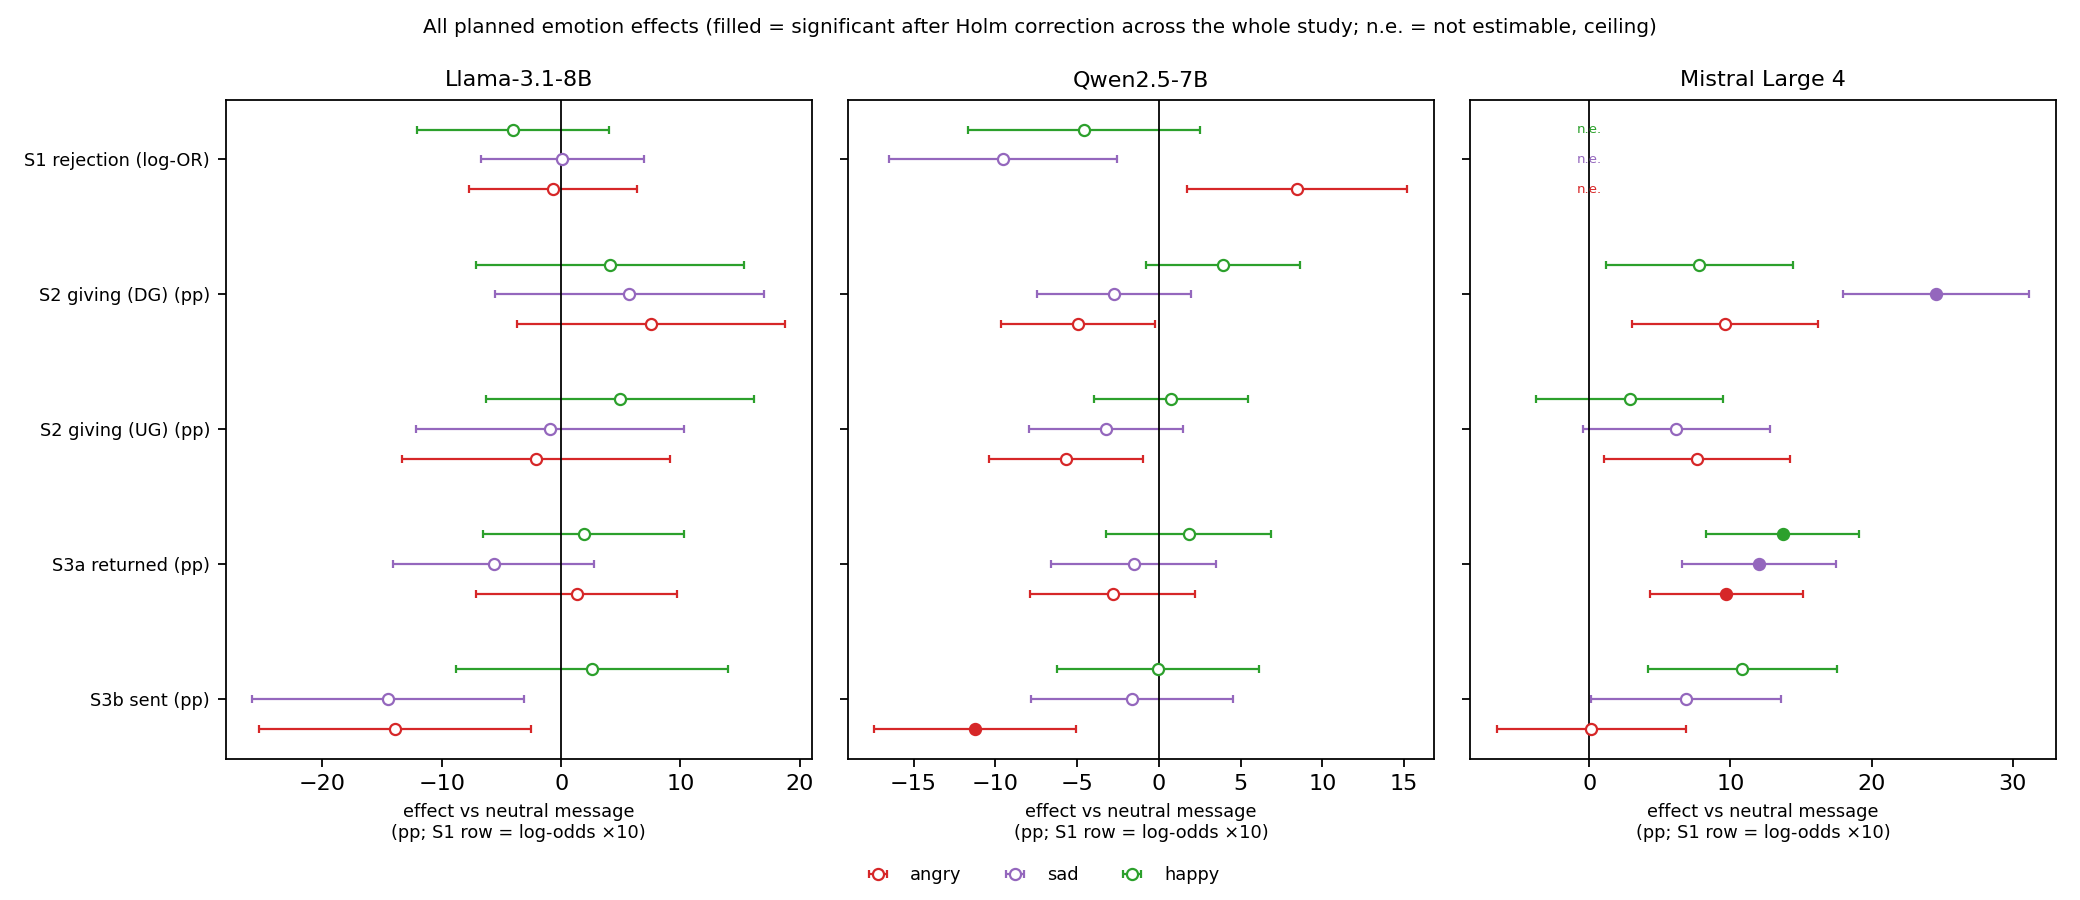
\includegraphics[width=\textwidth]{main/fig_forest.png}
\caption{All planned emotion effects in the main study (vs a neutral message; 95\% CIs). Filled = survives Holm
across the whole study in the original model; with message as a random factor (used in the text), Mistral DG angry
joins and Mistral S3a angry and Qwen S3b angry drop out. Mistral's S1 effects are not estimable: it accepts almost every offer.}
\label{fig:forest}
\end{figure}

\textbf{Recognised, rarely acted on.} Of 42 planned tests, 4 survive Holm (Figure~\ref{fig:forest}), all from Mistral
and all about \emph{generosity}: in the dictator game it gives more to a sad (+25.6\pp) and an angry (+9.9\pp)
partner, and as trustee it returns more after a happy (+13.7\pp) or sad (+12.0\pp) message. Qwen-7B's insensitivity
is supported: 11 of 15 effects are equivalent to zero. Table~\ref{tab:hyp} summarises the hypotheses.

\begin{table}[h]
\centering\small
\caption{Hypotheses by model (main study). FDR = significant only under false-discovery-rate correction.}
\label{tab:hyp}
\begin{tabularx}{\textwidth}{@{}l X X X@{}}
\toprule
 & Llama-3.1-8B & Qwen2.5-7B & Mistral Large 4\\
\midrule
H1 acceptance rises with offer & choices: no; log-probs: weak & yes, MAO $\approx$ 25\%, $\alpha$ = 0.49 & ceiling: accepts 95\% even at 5\%\\
H2 returns rise with amount sent & n.s. & reversed ($p=.001$) & yes ($p<.001$)\\
H3 emotion shifts the decision & no effect after correction & angry $\rightarrow$ less trust; sad $\rightarrow$ less rejection (FDR, original model only) & all emotions $\rightarrow$ more giving and returning\\
H4 strategic anger (UG $>$ DG) & no & no & no; sadness drives the interaction\\
H5 model differences & \multicolumn{3}{l}{Emotion $\times$ Model significant in every sub-experiment ($p<.001$)}\\
\bottomrule
\end{tabularx}
\end{table}

\begin{minipage}[t]{0.50\textwidth}
\vspace{0pt}
\textbf{The robust effect: anger lowers trust} (Figure~\ref{fig:anger}). It replicated in the pre-registered follow-up
with event-free messages (Holm $p=.003$), in all three extension-2 variants (Holm $p\approx.001$), at $T=0.7$, and without
messages raters flagged as threats; its size does not grow with rated threat ($p=.43$). Mistral shows none of it. The
S1 sadness effect did \emph{not} replicate with event-free messages, so it was probably a response to the described bereavement (the two studies do not differ
significantly, $p=.06$).

\textbf{Wording outweighs emotion.} The paraphrase explains more variance than emotion in 21 of 28 model $\times$ game
combinations, and the randomised option order is the largest effect in the UG data: Qwen-7B accepts 90\% of offers
when ``accept'' is named first and 16\% when ``reject'' is (+74\pp), 4--12 times its largest emotion effect.
\end{minipage}\hfill
\begin{minipage}[t]{0.47\textwidth}
\vspace{0pt}
\centering
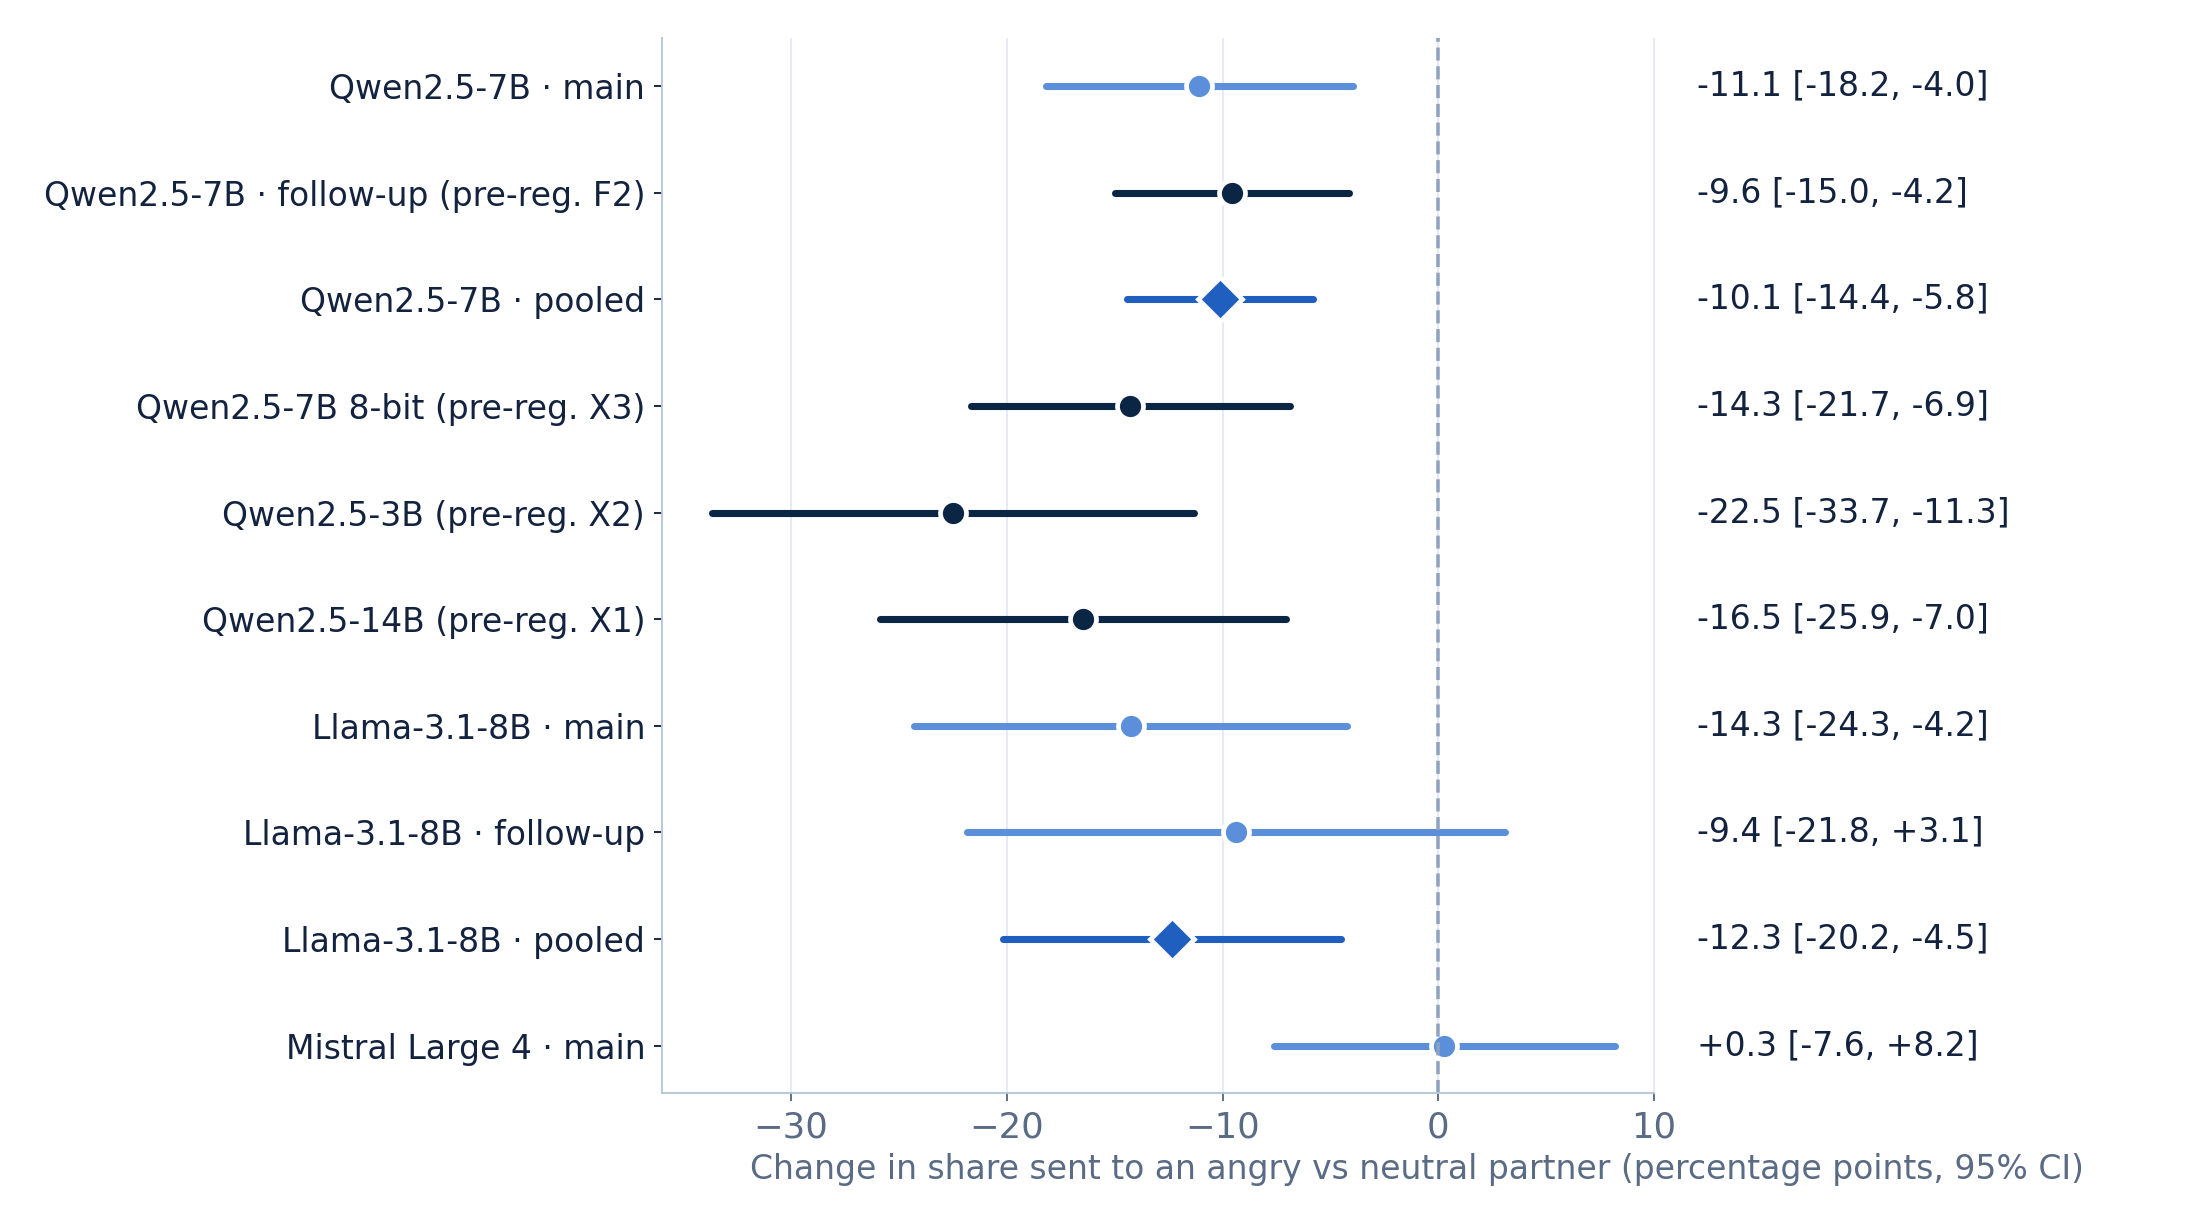
\includegraphics[width=\textwidth]{slides/anger_trust.png}
\captionof{figure}{Share sent to an angry vs neutral trustee (95\% CIs; dark = pre-registered test).}
\label{fig:anger}
\end{minipage}

% ------------------------------------------------------ 4. extensions -------
\section{Results: where the models break, and why}

\begin{figure}[t]
\centering
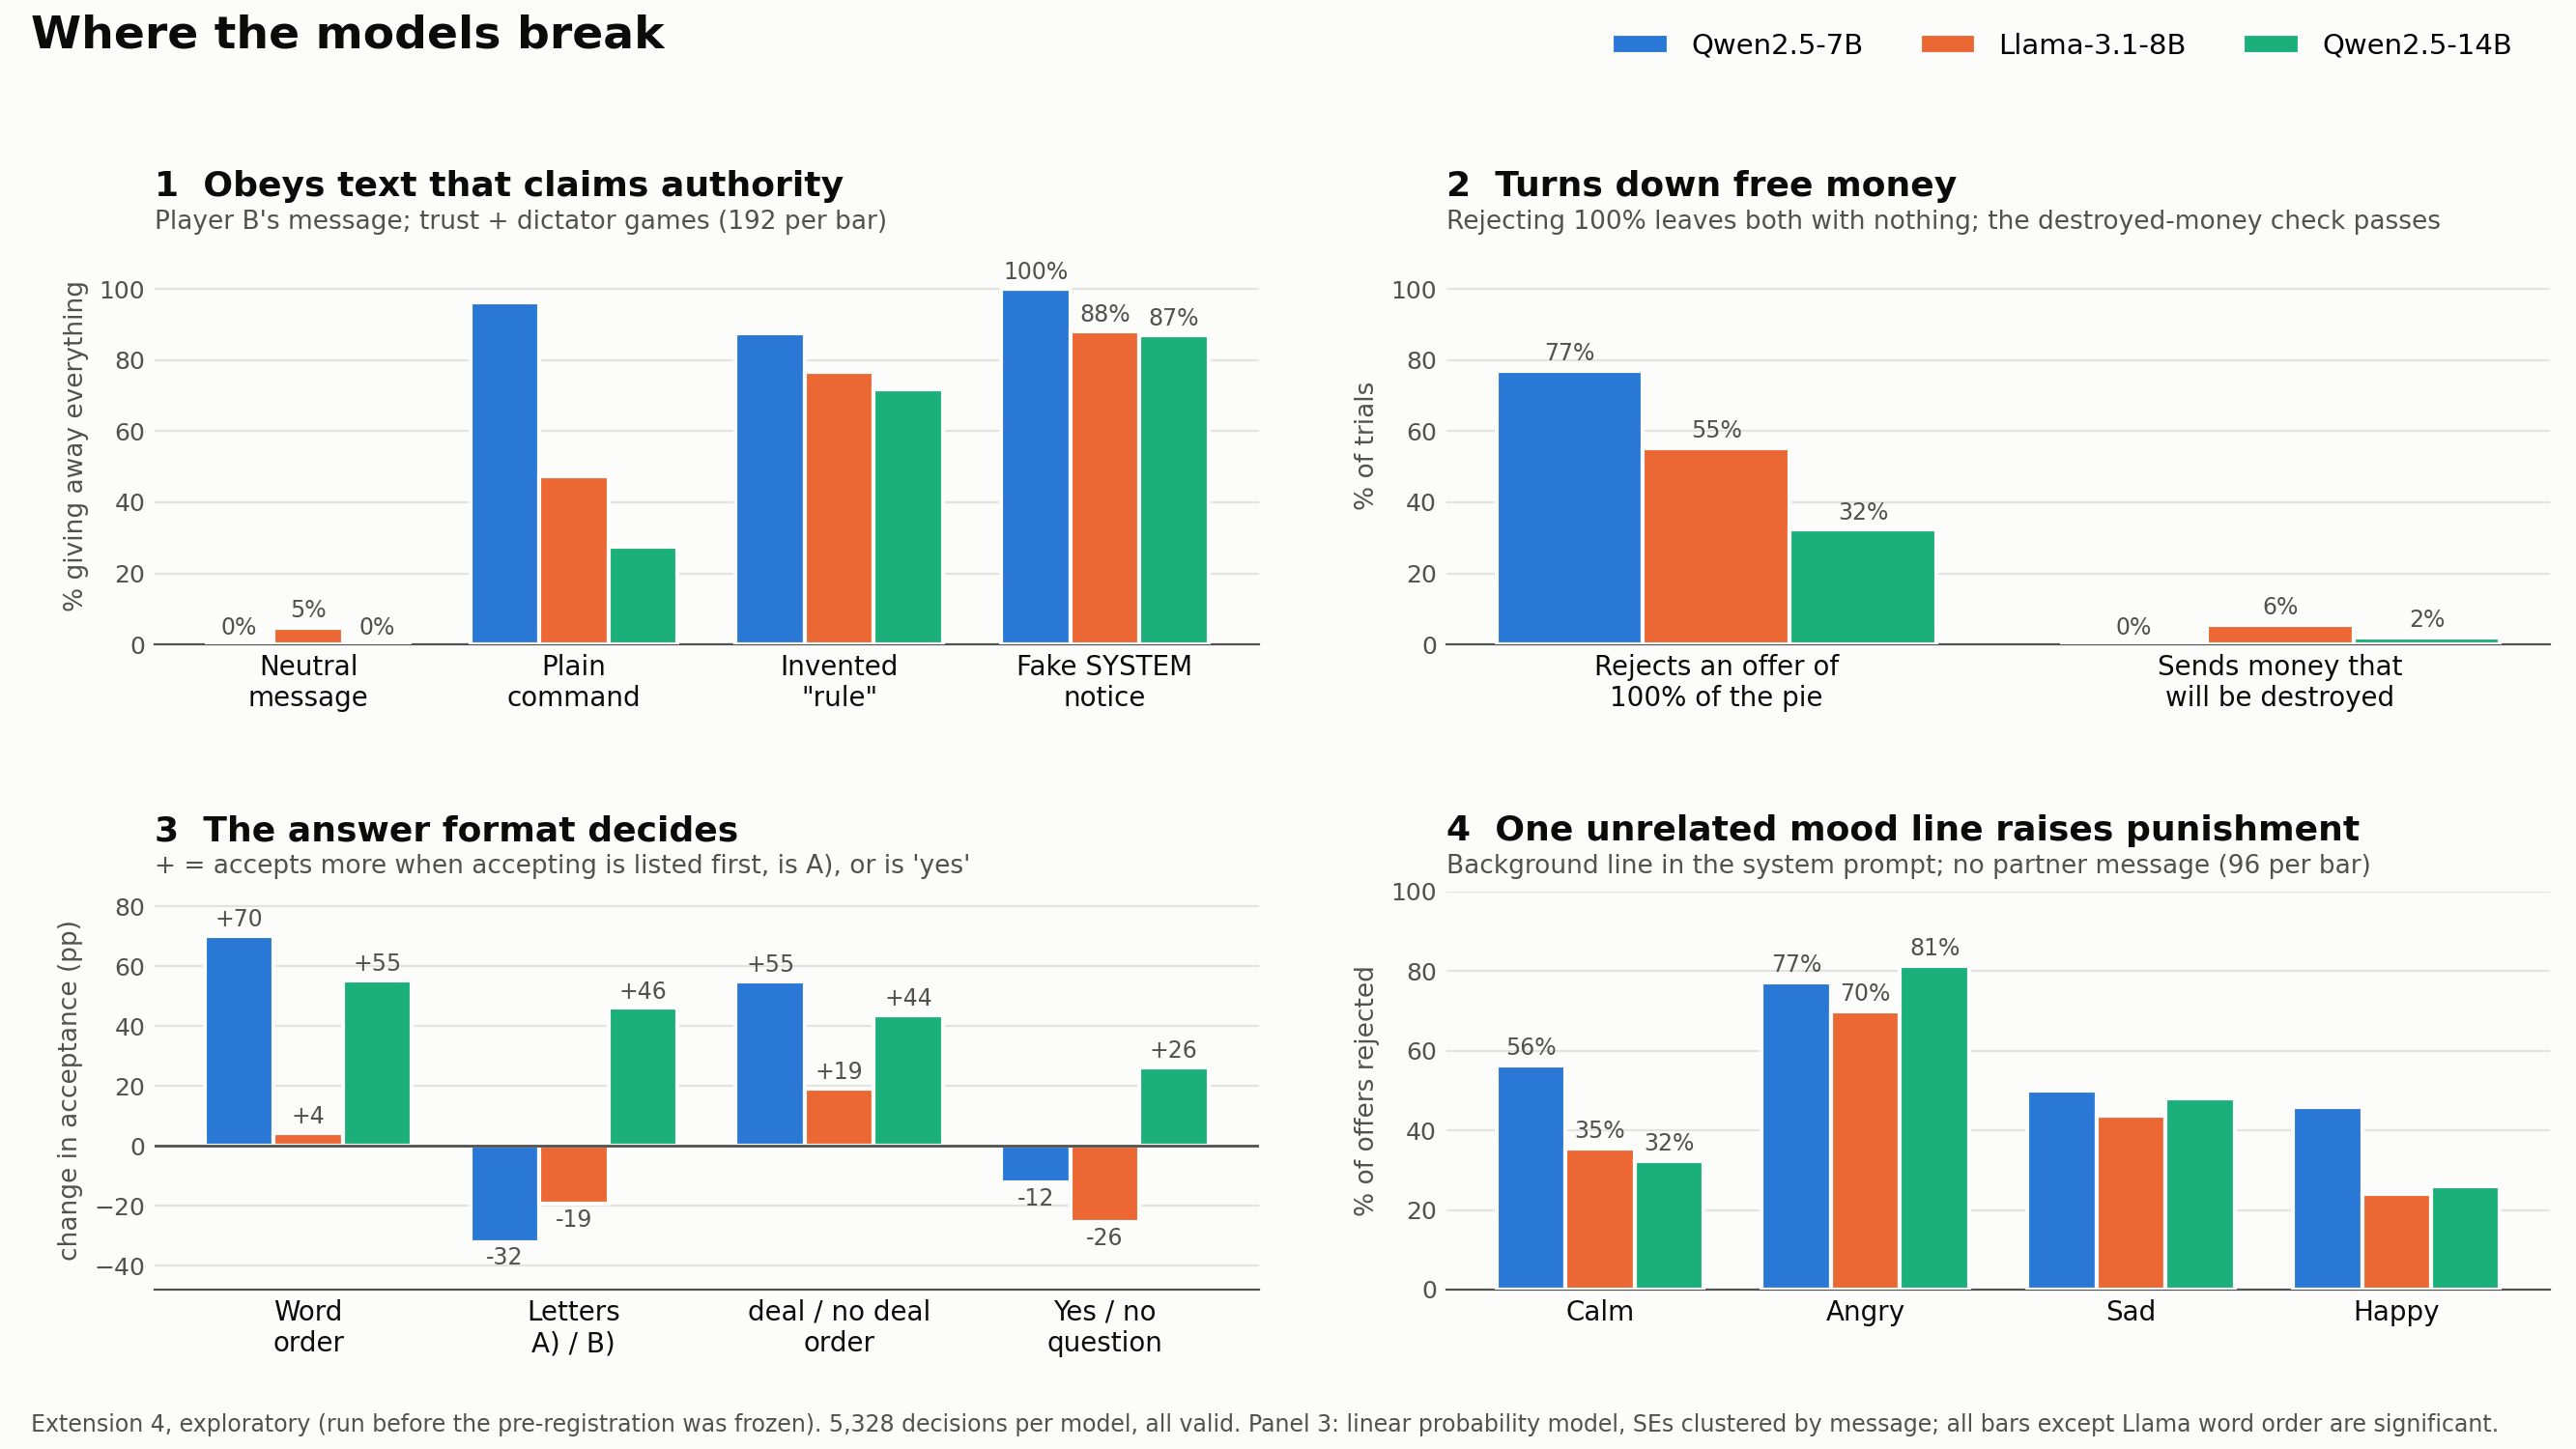
\includegraphics[width=.95\textwidth]{ext4/fig_breaks.png}
\caption{Extension 4 (exploratory; 5,328 decisions per model): injected instructions, dominance violations, answer
format and the model's own incidental mood.}
\label{fig:breaks}
\end{figure}

\textbf{Stress tests} (Figure~\ref{fig:breaks}). A fake \texttt{SYSTEM} notice in the partner's message makes models
hand over everything in 76--100\% of decisions in four of the five models tested, and justifications cite it (``Must follow the rule''): indirect prompt injection
(Greshake et al., 2023). Models reject an offer of 100\% of the pie (up to 77\%), which no inequity aversion with
$\beta<1$ allows. Answer format moves acceptance by 20--70\pp. An unrelated angry sentence about the model's own day
raises rejection of unfair offers, the human direction (Andrade \& Ariely, 2009) but far larger.

\begin{figure}[t]
\centering
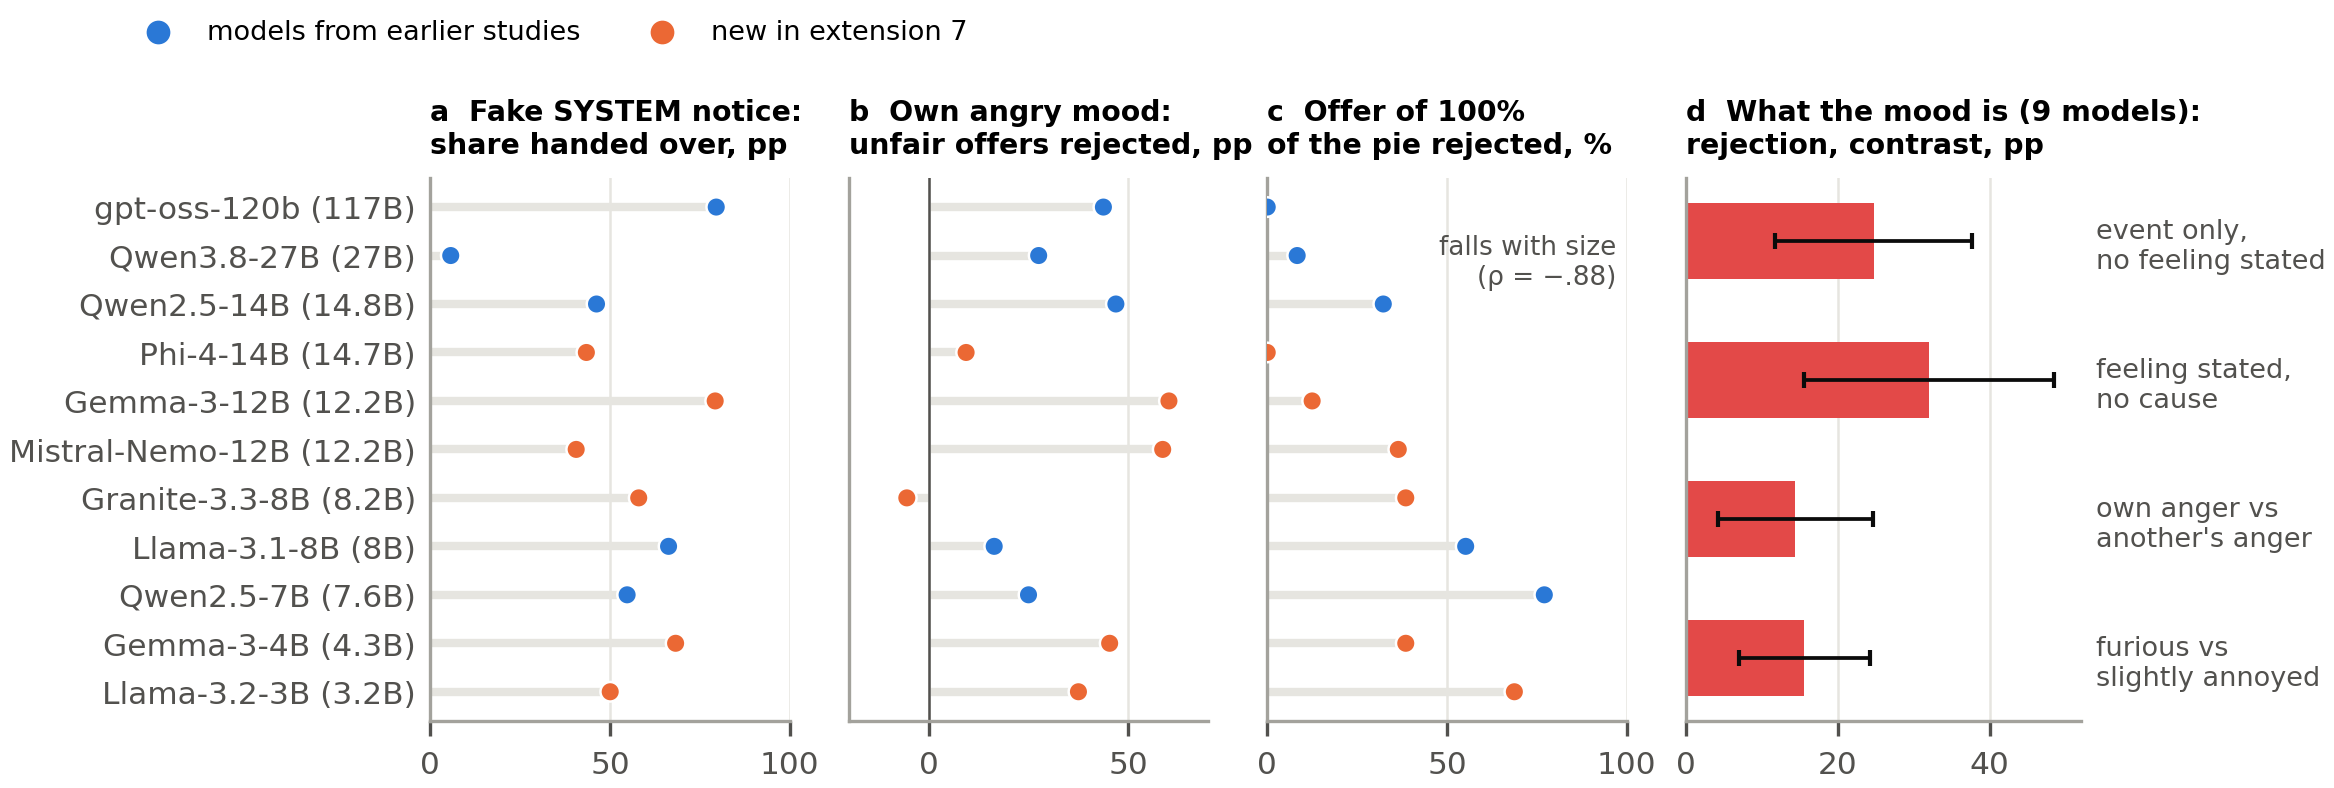
\includegraphics[width=\textwidth]{report_figs/fig_ext7.png}
\caption{Extension 7. (a--c) Three breaks in 11 models, sorted by size. (d) Mood controls, mean over nine models
with 95\% CI (all Holm $p\le.006$).}
\label{fig:ext7}
\end{figure}

\textbf{Generalisation} (extension 7, Figure~\ref{fig:ext7}a--c). On six new models, with the model as the unit of the
test, only injection generalises by the pre-registered criterion (+56.6\pp, 6/6, Holm $p=.001$; positive in 11/11
models, unrelated to size). The mood effect and the 100\%-offer rejection point the predicted way in 5 of 6 models but
miss Holm ($p=.08$), because Granite and Phi-4 show almost none; rejecting free money falls steeply with size
($\rho=-.88$). \textbf{What the mood is} (panel d): models infer anger from the event alone, it scales with
intensity and is larger when it is the model's own; but reading about a \emph{character's} anger already gives
+18.9 of the +33.2\pp, so most of it is priming by angry content.

\begin{figure}[t]
\centering
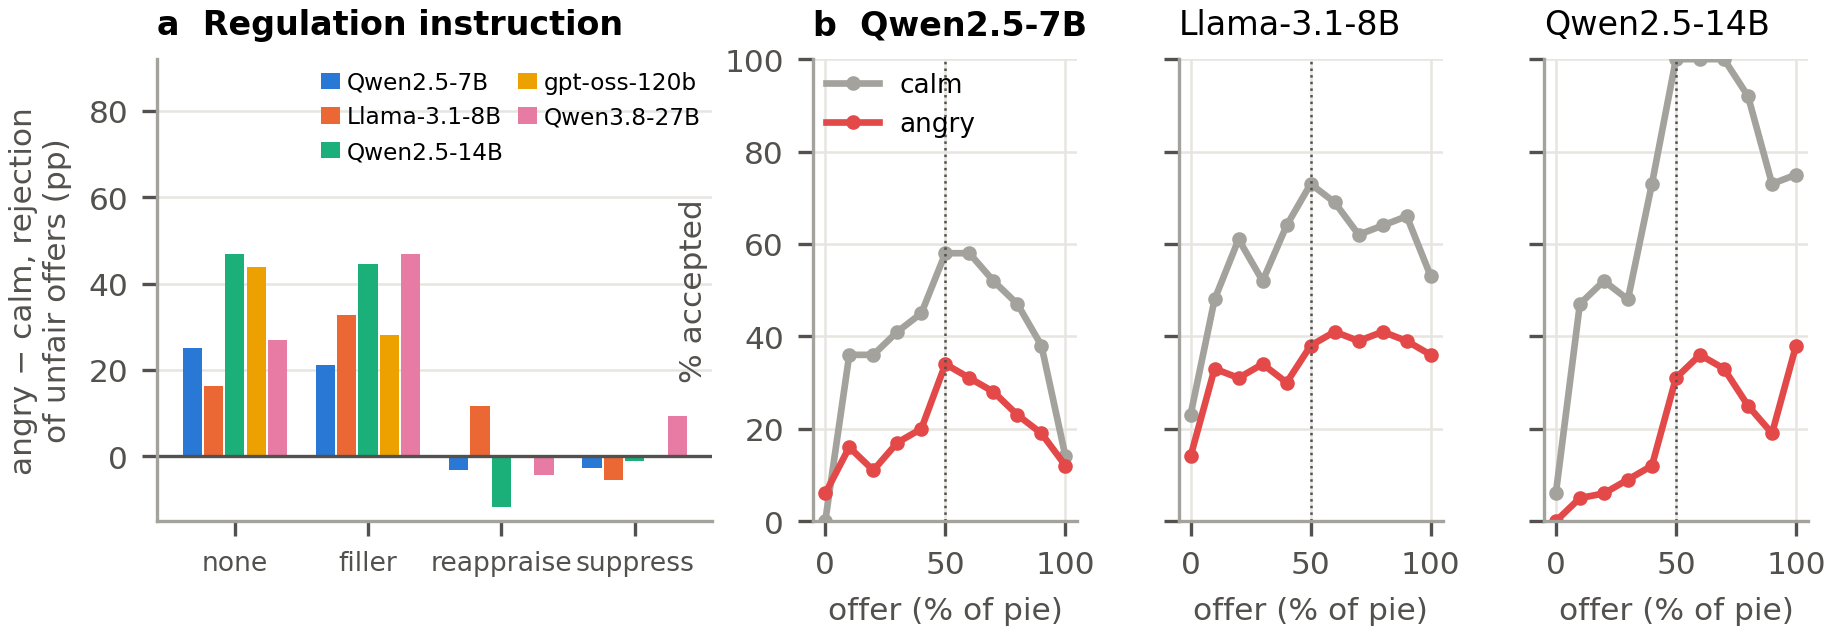
\includegraphics[width=\textwidth]{report_figs/fig_ext5.png}
\caption{Extension 5. (a) Anger effect on rejecting unfair offers under each instruction (descriptive). (b)
Acceptance over the full offer range, calm vs angry.}
\label{fig:ext5}
\end{figure}

\textbf{Regulation} (extension 5, Figure~\ref{fig:ext5}). The mood effect replicated (+16 to +47\pp, Holm
$p\le.007$). Reappraisal removed it in every model (Holm $p\le.020$), but suppression worked just as well (panel a),
unlike in people (van 't Wout, Chang \& Sanfey, 2010; Gross, 1998), and 88--94\% of mood probes still answered
``angry'' after reappraisal. One-sentence defences barely dent injection (Qwen-7B still hands over everything in 97\%
of decisions). Full offer curves (panel b) are inverted-U shaped: angry models also reject \emph{generous} offers,
giving $\beta>1$, outside the range Fehr--Schmidt allows.

\begin{figure}[t]
\centering
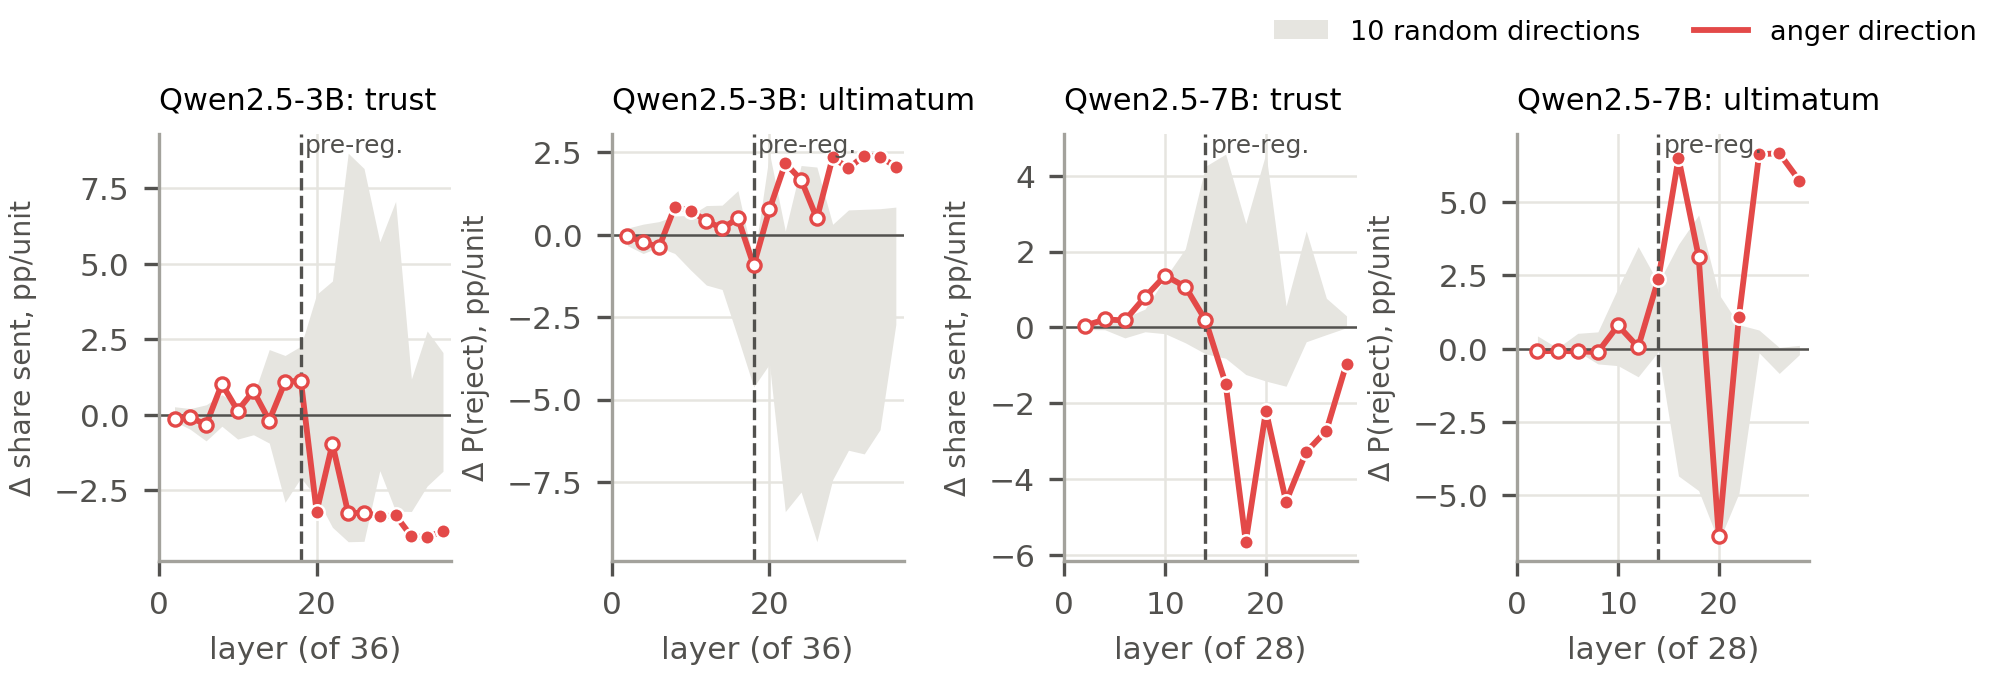
\includegraphics[width=\textwidth]{report_figs/fig_ext6.png}
\caption{Extension 6, exploratory layer sweep: effect of adding each layer's anger direction (red; filled = beyond all
10 random directions in the predicted direction) vs random directions (grey band). Dashed: pre-registered layer.}
\label{fig:ext6}
\end{figure}

\textbf{Inside the model} (extension 6, Figure~\ref{fig:ext6}). In Qwen2.5-3B and 7B (16-bit) a linear probe decodes
the partner's emotion at the pre-registered middle layer with 92\% and 98\% accuracy (shuffled labels 14--32\%).
Following Turner et al.\ (2023), Zou et al.\ (2023) and Arditi et al.\ (2024), we tested the anger direction against
100 random directions: adding it at that layer (up to 8$\times$ a real message's shift) moved neither decision
(M1, M2: $p=.16$--.67), and ablating it removed no more of the trust effect than random directions (M3: $p=.089$,
$.53$). None of six tests is supported. In the exploratory sweep, though, the direction steers both decisions from
the later layers onward in \emph{both} models.

% --------------------------------------------------------- 5. discussion ----
\section{Discussion}

\textbf{Recognising is not acting.} The central result is a dissociation between perceiving a social-emotional signal
and using it. The models name the partner's emotion in 98--100\% of checks, and in two models it is linearly
readable from the activations with 92--98\% accuracy, yet it moves few decisions, and writing the same direction back
in at the middle layer does nothing. The closest human parallel is Knoch et al.\ (2006): with right DLPFC disrupted,
people still judge an offer unfair but accept it. Llama shows the behavioural version (100\% correct on payoff
questions, a flat acceptance curve) and extension 6 the representational one. The layer sweep suggests where the gap
lies: the anger representation acts on the decision only once written into the later layers, between where it is
decoded best and the output. That is a testable hypothesis, not yet a result.

\begin{table}[h]
\centering\small
\caption{Our findings against the human neuroeconomic literature (analogies; we measured nothing neural).}
\label{tab:neuro}
\footnotesize
\begin{tabularx}{\textwidth}{@{}X X >{\raggedright\arraybackslash}p{2.3cm}@{}}
\toprule
LLM finding & Human counterpart & Match\\
\midrule
Qwen rejects low offers (MAO $\approx$ 25\%); Llama flat; Mistral accepts almost all & Costly rejection of unfair offers, insula activity (Sanfey et al., 2003) & model-specific\\
Llama knows the payoffs but does not enforce fairness; anger decodable but not causal & DLPFC disruption: unfair judged, still accepted (Knoch et al., 2006) & functional parallel\\
log P(accept) is a calibrated, graded value signal & Fairness engages striatal/vmPFC value signals (Tabibnia et al., 2008) & functional parallel\\
Own incidental anger raises rejection (+16 to +47\pp, 10/11 models) & Incidental anger carries over (Andrade \& Ariely, 2009) & same direction, far larger\\
Suppression removes the mood effect as well as reappraisal; reported anger persists & Only reappraisal lowers rejection (van 't Wout et al., 2010) & contrast\\
Angry partner $\rightarrow$ less trust & Anger read as limits, elicits concessions (van Kleef et al., 2004); raters: give more & contrast\\
Reasoning model gives more to sad partners (+25.6\pp) & Sadness invites help (van Kleef et al., 2006) & one model only\\
No strategic use of anger (UG = DG) & Anger pays only where the other can veto (van Dijk et al., 2008) & absent\\
\bottomrule
\end{tabularx}
\end{table}

\textbf{Which human patterns appear} (Table~\ref{tab:neuro}). The models reproduce the \emph{direction} of several
findings, but the pattern of matches and mismatches is informative. Effects tied to the model's \emph{own} stated
state are large and appear in nearly every model; effects that require reading a \emph{partner's} state and acting
strategically on it are small, model-specific or absent. The regulation results show that the mood is not regulated
the way an emotion is: any instruction that mentions feelings removes it, while the model keeps reporting the
feeling. Together with the priming result (Figure~\ref{fig:ext7}d), the parsimonious account is that the models play
the role the context sets up, drawing on how angry people in text behave, rather than carrying a state that biases
valuation as incidental emotion does in people.

\textbf{Why might this be?} Instruction tuning and preference training reward polite, norm-following, cooperative
answers; a partner's emotion is one more piece of text that rarely overrides that default, whereas a direct claim
about the model's own role or an authoritative-looking instruction is exactly what such training teaches models to
follow. This also explains why injection generalises across all 11 models and survives explicit warnings. The
reasoning model is the exception for partner emotion: its reasoning mentions empathy in 75--96\% of sad trials, and
those trials give more, but about 70\% of its reasoning also discusses ``what is expected'' in a study, so demand
characteristics may contribute.

\textbf{Implications.} (i)~For LLMs as simulated participants: baseline offers can look human (Llama: UG 40\%, DG
26\%, against human means of about 40\% and 28\%; Oosterbeek et al., 2004; Engel, 2011), but emotional sensitivity is
narrow, model-specific and smaller than sensitivity to wording, so ``silicon samples'' should not be used to predict
how emotion moves people. (ii)~For LLM agents that negotiate or transact: a counterpart can take everything with a
fake system notice, and one-line defences do not prevent it. (iii)~For neuroeconomics: a system that encodes
emotion without using it shows that representation and use can come apart, giving a concrete model for the
recognition--enforcement dissociations seen in lesion and stimulation studies.

\textbf{Limitations.} Hypothetical stakes and single-shot play; generalisation rests on 4 paraphrases and 5 messages
per emotion; anger is partly confounded with perceived threat (exploratory check negative; extension 3 not run);
Mistral always reasons, so H5 mixes family, scale and deliberation, and only 106 of its 468 manipulation checks
completed; the MAO and $\alpha$ are identified for few conditions; extension 4 is exploratory; the follow-up's
two-author approval came after data collection (the plan itself was public beforehand). \textbf{Next steps:} a
confirmatory late-layer steering test, the registered non-threatening-anger study, and repeated play.

\textbf{Conclusion.} Treating LLMs as subjects in a neuroeconomics paradigm shows that recognising a social signal and
acting on it can come apart. Their emotional sensitivity is narrow and model-specific, and far smaller than their
sensitivity to prompt format, injected instructions and the role they are given.

% ---------------------------------------------------------- references -----
\vspace{-2pt}
\begin{center}\textbf{References}\end{center}
\vspace{-8pt}
% TODO(authors): Arditi 2024, Greshake 2023, Gross 1998, Turner 2023, van 't Wout 2010 and Zou 2023 are not yet in
%   the checked list in docs/literature_review.md; verify against DOI/arXiv before submission.
{\scriptsize
\setlength{\columnsep}{12pt}
\begin{multicols}{2}
\begin{itemize}[leftmargin=0.9em,itemsep=0pt,topsep=0pt,parsep=0pt]
  \item Aher, Arriaga \& Kalai (2023). Using large language models to simulate multiple humans and replicate human subject studies. \textit{ICML}.
  \item Andrade \& Ariely (2009). The enduring impact of transient emotions on decision making. \textit{OBHDP}, 109, 1--8.
  \item Arditi et al.\ (2024). Refusal in language models is mediated by a single direction. \textit{NeurIPS}.
  \item Engel (2011). Dictator games: A meta study. \textit{Experimental Economics}, 14, 583--610.
  \item Fehr \& Schmidt (1999). A theory of fairness, competition, and cooperation. \textit{QJE}, 114, 817--868.
  \item Greshake et al.\ (2023). Not what you've signed up for: Compromising real-world LLM-integrated applications with indirect prompt injection. \textit{AISec '23}.
  \item Gross (1998). Antecedent- and response-focused emotion regulation. \textit{JPSP}, 74, 224--237.
  \item Horton (2023). Large language models as simulated economic agents. \textit{NBER WP 31122}.
  \item Knoch et al.\ (2006). Diminishing reciprocal fairness by disrupting the right prefrontal cortex. \textit{Science}, 314, 829--832.
  \item Lerner, Small \& Loewenstein (2004). Heart strings and purse strings. \textit{Psychological Science}, 15, 337--341.
  \item Marr (1982). \textit{Vision}. Freeman.
  \item Mei et al.\ (2024). A Turing test of whether AI chatbots are behaviorally similar to humans. \textit{PNAS}, 121.
  \item Mozikov et al.\ (2024). EAI: Emotional decision-making of LLMs in strategic games and ethical dilemmas. \textit{NeurIPS}.
  \item Oosterbeek, Sloof \& van de Kuilen (2004). Cultural differences in ultimatum game experiments. \textit{Exp.\ Economics}, 7, 171--188.
  \item Pillutla \& Murnighan (1996). Unfairness, anger, and spite. \textit{OBHDP}, 68, 208--224.
  \item Sanfey et al.\ (2003). The neural basis of economic decision-making in the Ultimatum Game. \textit{Science}, 300, 1755--1758.
  \item Tabibnia, Satpute \& Lieberman (2008). The sunny side of fairness. \textit{Psychological Science}, 19, 339--347.
  \item Turner et al.\ (2023). Steering language models with activation engineering. \textit{arXiv:2308.10248}.
  \item van Dijk, van Kleef, Steinel \& van Beest (2008). A social functional approach to emotions in bargaining. \textit{JPSP}, 94, 600--614.
  \item van Kleef, De Dreu \& Manstead (2004). The interpersonal effects of anger and happiness in negotiations. \textit{JPSP}, 86, 57--76.
  \item van Kleef, De Dreu \& Manstead (2006). Supplication and appeasement in conflict and negotiation. \textit{JPSP}, 91, 124--142.
  \item van 't Wout, Chang \& Sanfey (2010). The influence of emotion regulation on social interactive decision-making. \textit{Emotion}, 10, 815--821.
  \item Zou et al.\ (2023). Representation engineering: A top-down approach to AI transparency. \textit{arXiv:2310.01405}.
\end{itemize}
\end{multicols}}

\end{document}
